\documentclass{article}
\usepackage{graphicx}
\usepackage[margin=1.5cm]{geometry}
\usepackage{amsmath}

\begin{document}
\twocolumn

\title{Friday Warm Up: Vectors and Kinematics I, II}
\author{Prof. Jordan C. Hanson}

\maketitle

\section{Memory Bank}

\begin{enumerate}
\item $\vec{v} = v_x \hat{i} + v_y \hat{j}$ ... The $\hat{i}$ and $\hat{j}$ components of a vector
\item $|\vec{v}| = \sqrt{v_x^2 + v_y^2}$ ... The magnitude of the vector
\item $v_x = |\vec{v}| \cos\phi$, $v_y = |\vec{v}| \sin\phi$ ... The x and y-components of the vector
\item $\vec{v} = d\vec{x}/dt$ ... Definition of velocity.
\item $\vec{a} = d\vec{v}/dt$ ... Definition of acceleration.
\end{enumerate}

\begin{figure}
\centering
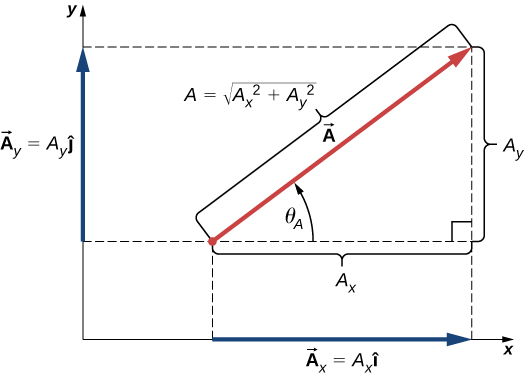
\includegraphics[width=0.24\textwidth]{figures/vector1.jpeg}
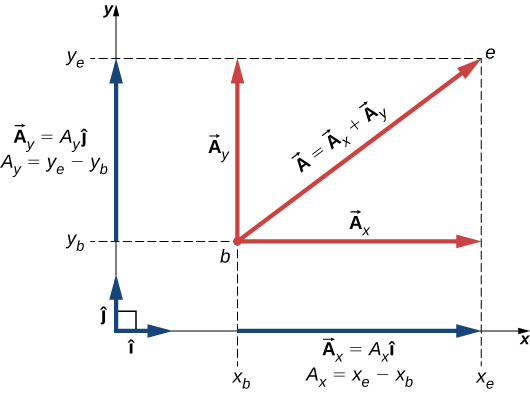
\includegraphics[width=0.24\textwidth]{figures/vector2.jpeg}
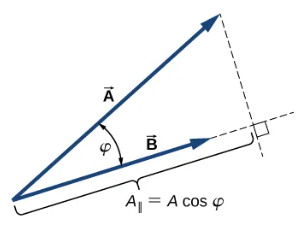
\includegraphics[width=0.24\textwidth]{figures/projection_2.png}
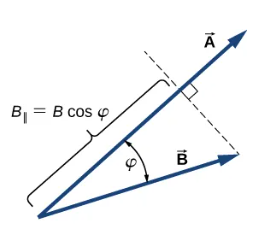
\includegraphics[width=0.24\textwidth]{figures/projection_1.png}
\caption{\label{fig:1} (Top left) A vector broken into $\hat{i}$ and $\hat{j}$ components. (Top right) Adding those components produces the vector. (Bottom left) The dot-product $\vec{A} \cdot \vec{B}$ gives the projection of $\vec{A}$ along $\vec{B}$, or (Bottom right) $\vec{B}$ along $\vec{A}$.}
\end{figure}

\section{Chapter 2 - Kinematics I}

\begin{enumerate}
\item Suppose a microbe is trapped in a 2D microscope slide and is observed to move randomly, beginning at the origin.  Determine the final location, if it has the following displacements:
\begin{itemize}
\item $\Delta\vec{x}_1 = 3\hat{i}+3\hat{j} ~~$mm
\item $\Delta\vec{x}_1 = -1\hat{i}-1\hat{j} ~~$mm
\item $\Delta\vec{x}_1 = 2\hat{i}-2\hat{j} ~~$mm
\item $\Delta\vec{x}_1 = -4\hat{i}+4\hat{j} ~~$mm
\end{itemize}
\item (a) Draw the trajectory of the microne in a 2D coordinate system.  (b) If the time duration for this trajectory is 50 ns, what is the average velocity? \\ \vspace{3cm}
\item For the microbe in Exercises 1 and 2, give the magnitude and angle of the final displacement. \\ \vspace{2cm}
\item Let $t$ represent time (seconds), and $\vec{x}$ represent displacement (meters).  Suppose the path of a system is
\begin{equation}
\vec{x} = -2.0 t^2 \hat{j} + 4.0 t \hat{i} + 80.0 \hat{j}~~(m)
\end{equation}
(a) Where is the system at $t=0$? (b) What is the velocity vector of the system? (c) What is the velocity at $t=2$ seconds? (d) What is the acceleration? \\ \vspace{2.5cm}
\item Suppose sunshine is coming straight down and a palm tree casts a shadow on the beach.  If the shadow of the palm is 12 meters long, and the angle of the palm is 60 degrees with respect to the beach, how long is the palm?
\end{enumerate}

\end{document}
